\documentclass[12pt,a4paper]{report}

\usepackage{cmap}
\usepackage[warn]{mathtext}
\usepackage[english,russian]{babel}
\usepackage{indentfirst}
\usepackage{amsmath}
\usepackage{amsfonts}
\usepackage{amssymb}
\usepackage{graphicx}
\graphicspath{{image/}}
\usepackage{listings}
\usepackage{hyperref}
\usepackage{float}
\usepackage{fontspec}
\usepackage{placeins}
\setmainfont{Times New Roman}
\setmonofont{Arial}

\lstset{
	inputencoding=utf8x,
	extendedchars=\true,
	frame=single,
	breaklines=true,
	numbers=left,
	keepspaces = true}

\voffset -24.5mm
\hoffset -5mm
\textwidth 173mm
\textheight 240mm
\oddsidemargin=0mm \evensidemargin=0mm


\begin{document}
	\begin{titlepage}
\begin{center}

\textbf{Санкт-Петербургский политехнический университет Петра Великого}

\vspace{5mm}
Институт компьютерных наук и технологий

\vspace{5mm}
Кафедра компьютерных систем и программных технологий

\vspace*{\fill}

\huge{Курсовой проект}

%\Large{о лабораторной работе №1}

\large{по дисциплине: <<Проектирование операционных систем>>}

\vspace*{2mm}
\large{Тема: <<Разработка мобильного оконного менеджера>>}

\vspace*{\fill}
\end{center}

%\begin{flushright}
\begin{large}
\hspace{0.4\linewidth} \textbf{Работу выполнил студент}

\vspace{5mm}
\hspace{0.4\linewidth} 13541/4 \hspace{1cm} \textit{Абдуллин А. М.}

\vspace{3mm}
\hspace{0.4\linewidth} \textbf{Преподаватель}

\vspace{5mm}
\hspace{0.4\linewidth} \underline{\hspace{2cm} } \hspace{3mm} \textit{Душутина Е.В.}
\end{large}
%\end{flushright}

\vspace*{3cm}

\begin{center}
\normalsize Санкт-Петербург\\2017
\end{center}
\end{titlepage}
	\renewcommand{\thesection}{\arabic{section}}
	\setcounter{page}{2}
	\tableofcontents
	\pagebreak
	
	\setcounter{totalnumber}{10}
	\setcounter{topnumber}{10}
	\setcounter{bottomnumber}{10}
	\renewcommand{\topfraction}{1}
	\renewcommand{\textfraction}{0}
	
	\documentclass[11pt,a4paper]{extarticle}
\usepackage[left=3cm, right=1cm, top=2cm, bottom=2cm]{geometry}
\usepackage[utf8]{inputenc}
\usepackage[russian]{babel}
\usepackage[OT1]{fontenc}
\usepackage{amsmath}
\usepackage{amsfonts}
\usepackage{amssymb}
\usepackage{graphicx}
\usepackage{listings}
\graphicspath{{image/}}
\bibliographystyle{plain}
\begin{document}
\large{\textbf{Техническое задание}}

Необходимо создать мобильный оконный менеджер (ОМ). Конечной целью работы является запуск созданного ОМ на платформе Raspberry Pi Zero. Из-за малой мощности необходимо, чтобы ОМ работал на протоколе Wayland.

Wayland --- протокол для организации графического сервера в Linux и других UNIX-подобных операционных системах, а также его библиотечная реализация в Си. В роли клиента может выступать пользовательское приложение, X сервер или другой дисплейный сервер. 
\begin{itemize}
\item Цель: радикально упростить графическую среду Linux по сравнению с X Window System.
\item Использует Unix Domain Sockets, сетевой прозрачности нет. 
\item Главным образом использует DRI (Direct Rendering Infrastructure) --- интерфейс доступа к видеоаппаратуре. 
\item Устройства ввода-вывода управляются полностью из ядра. 
\item Распределение буфера и отрисовка полностью на стороне клиента.
\end{itemize}

\begin{figure}[h!]
\center
\includegraphics[width=\linewidth]{image/wayland-architecture}
\caption{Архитектура Wayland}
\label{img:wayland-architecture}
\end{figure}

Как показано на рисунке \ref{img:wayland-architecture}, ключевым понятием в архитектуре Wayland является композитор. Композитор --- это дисплейный сервер, который взаимодействуют с пользовательскими устройствами ввода-вывода, с железом, управляет потоком данных клиентских программ. В конечном счете композитор работает с буферами вывода всех отображаемых окон, определяет как эти буфера будут располагаться в буфере вывода дисплея. В X Window System функциональность композитора была вынесена в реализацию сервера (X Server), ОМ ничего об этом не знал. Однако, в ОМ для Wayland реализация композитора это один из основных этапов разработки. Так как реализация собственного композитора является очень объемной и сложной задачей (даже простейшие композиторы занимают ~ 10-15к строк кода), было решено при реализации ОМ использовать какую-либо библиотеку, содержащую в себе композитор. Таким образом, задача созданного ОМ будет заключаться в управлении пользовательскими окнами.

Так же было сказано, что конечной целью разработки является запуск ОМ на Raspberry Pi Zero. Однако, RPi имеет свою проприетарную графику, которая не поддерживается существующими композиторами и оконными менеджерами. Как было указано выше, Wayland использует DRI (для обеспечения аппаратного ускорения с использованием Mesa3D). Таким образом, необходимо настроить RPi для представления его графического устройства в виде DRM (Direct Rendering Manager). Для этого необходимо настроить драйвер VC4 для RPi. VC4 --- это драйвер, включенный в пакет Mesa3D, который позволяет представить проприетарное графическое устройство RPi в виде стандартного DRM устройства.

Мобильный оконный менеджер должен так же иметь два встроенных системных приложения:
\begin{itemize}
\item Строка состояния, которая отображает информацию об устройстве (текущее время, уровень заряда, уровень сигнала и т.д.). Строка состояния всегда отображается в верхней части экрана.
\item Рабочий стол, на котором расположены иконки запуска приложений, установленных в системе. Рабочий стол отображается на всю часть экрана, не занятую строкой состояния.
\end{itemize}
Данные системные приложения не являются непосредственной частью ОМ. ОМ автоматически запускает их при своем запуске, и запоминает их PID для соответствующего их отображения. В ОМ должна присутствовать возможность конфигурирования. В частности: возможность указать путь к приложениям строки состояния и рабочего стола.

При запуске несистемных приложений ОМ скрывает рабочий стол, выводит запущенное приложение на передний план и делает его активным. Так же ОМ должен поддерживать три типа окон:
\begin{itemize}
\item обычные окна приложений, которые отображаются во весь экран
\item всплывающие уведомления (например, контекстное меню при нажатии правой кнопки мыши), которые отображаются в соответствии со своими размерами в указанной точке. Например, при нажатии на правую кнопку мыши открывается контекстное меню в точке нажатия с необходимыми размерами
\item окна меню (например стандартные меню типа "Файл" и т.д. в верхней части приложений). Должны запускаться в соответствии со своими размерами и отрисовываться начиная с нажатой кнопки.
\end{itemize}

Таким образом, задачу можно разделить на две практические независимые части:
\begin{enumerate}
\item Настройка ОС RPi для представления графического устройства в виде стандартного DRM
\item Разработка мобильного ОМ для Wayland:
	\begin{itemize}
	\item использование библиотеки-композитора
	\item поддержка системных приложений
	\item конфигурируемость ОМ
	\item поддержка и соответствующее отображение трех типов окон (обычное окно, всплывающее окно, окно меню)
	\end{itemize}
\end{enumerate}

\end{document}
	\section{Описание задачи}
Данная курсовая работа выполнена в раках проекта по разработке мобильного устройства  на платформе Raspberry Pi Zero~\cite{RPiZero}. Данный проект включает в себя несколько задач:
\begin{itemize}
\item разработка аппаратной платформы мобильного устройства на основе Raspberry Pi Zero --- подбор необходимых компонентов мобильного устройства (GSM модуль, динамик, микрофон, аккумулятор и т.д.) и их размещение на плате устройства
\item установка и конфигурирование ОС для Raspberry Pi
\item разработка стека драйверов для комплектующих
\item разработка сервисного слоя (в виде демонов UNIX), который будет предоставлять необходимую информацию клиентским приложениям
\item \textbf{разработка мобильного оконного менеджера}, который позволит запускать и отображать на экране графические пользовательские приложения
\item разработка клиентских приложений (для осуществления звонков, настроек и т.д.)
\end{itemize}

Архитектура разрабатываемого проекта приведена на рисунке~\ref{fig:architecture}.
\begin{figure}[h!]
\center{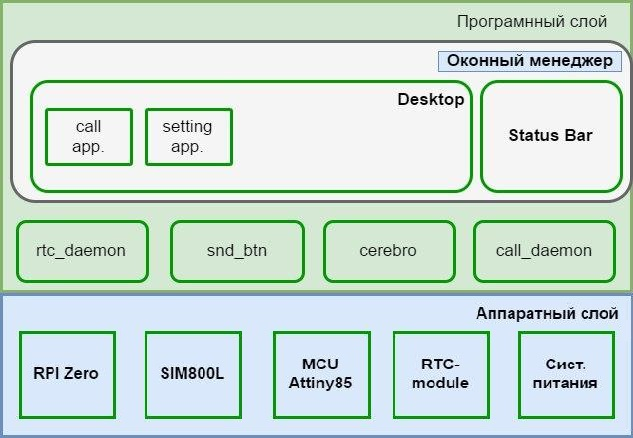
\includegraphics[width=\linewidth]{architecture}}
\caption{Архитектура проекта}
\label{fig:architecture}
\end{figure}

Таким образом, конечной целью разработки оконного менеджера~(ОМ) является его запуск на Raspberry Pi Zero. Необходимо учесть, что Raspberry обладает малой вычислительной мощностью, поэтому ОМ должен быть реализован как можно более оптимальным образом.

Мобильный ОМ должен так же иметь два встроенных системных приложения:
\begin{itemize}
\item строка состояния, которая отображает информацию об устройстве (текущее время, уровень заряда, уровень сигнала и т.д.). Строка состояния всегда отображается в верхней части экрана
\item рабочий стол, на котором расположены иконки запуска приложений, установленных в системе. Рабочий стол отображается на всю часть экрана, не занятую строкой состояния
\end{itemize}
Данные системные приложения не являются непосредственной частью ОМ. ОМ автоматически запускает их при своем запуске, и запоминает их идентификаторы для соответствующего отображения. ОМ должен иметь возможности указания путей к приложениям строки состояния и рабочего стола (т.е. должен иметь возможность конфигурирования).

При запуске несистемных приложений ОМ скрывает рабочий стол, выводит запущенное приложение на передний план и делает его активным. ОМ должен поддерживать три типа окон:
\begin{itemize}
\item обычные окна приложений, которые отображаются во весь экран
\item всплывающие уведомления (например, контекстное меню при нажатии правой кнопки мыши), которые отображаются в соответствии со своими размерами в указанной точке. Например, при нажатии на правую кнопку мыши открывается контекстное меню в точке нажатия с необходимыми размерами
\item окна меню (например стандартные меню типа "Файл" и т.д. в верхней части приложений). Должны запускаться в соответствии со своими размерами и отрисовываться начиная с нажатой кнопки.
\end{itemize}

Созданный оконный менеджер так же должен иметь возможность обработки управляющих комбинаций клавиш для:
\begin{itemize}
\item закрытия приложения
\item завершения работы ОМ
\item перелистывания окон
\item запуска терминала
\end{itemize}

Так же ОМ должен иметь возможности перемещения и изменения размеров окон.
	\section{Теоретические сведения}
\subsection{Протокол Х и X Window System}
X Window System --- оконная система, обеспечивающая стандартные инструменты и протоколы для построения графического интерфейса пользователя, используется в UNIX-подобных ОС. X Window System обеспечивает базовые функции графической среды: отрисовку и перемещение окон на экране, взаимодействие с устройствами ввода, такими как, например, мышь и клавиатура. X Window System не определяет деталей интерфейса пользователя --- этим занимаются оконные менеджеры. В X Window System предусмотрена сетевая прозрачность: графические приложения могут выполняться на другой машине в сети, а их интерфейс при этом будет передаваться по сети и отображаться на локальной машине пользователя. Архитектура протокола X приведена на рисунке~\ref{fig:xArchitecture}.
\begin{figure}[h!]
\center{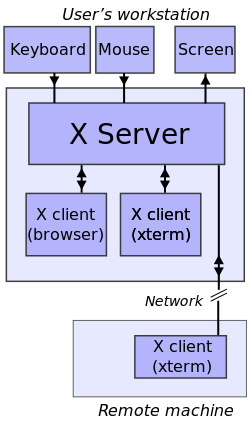
\includegraphics[width=0.6\linewidth]{xArchitecture}}
\caption{Архитектура протокола X}
\label{fig:xArchitecture}
\end{figure}

X использует модель клиент-сервер: сервер X взаимодействует с различными клиентскими программами. Сервер принимает запросы на графический вывод (окна) и отправляет обратно пользовательский ввод (с клавиатуры, мыши или сенсорного экрана). Сервер может работать как: 
\begin{itemize}
\item Приложение, отображающее окно другой системы отображения
\item Системная программа, управляющая видеовыходом ПК
\item Выделенный набор аппаратных средств
\end{itemize}

X рассматривает перспективу приложения, а не конечного пользователя: X предоставляет приложениям дисплей для отображения и пользовательский ввод-вывод приложениям, поэтому он является сервером; приложения используют эти службы, поэтому они являются клиентами. 

Протокол связи между сервером и клиентом работает прозрачно: клиент и сервер могут работать на одном компьютере или на разных устройствах, возможно, с разными архитектурами и операционными системами. Клиент и сервер могут даже безопасно обмениваться данными через Интернет путем туннелирования соединения по зашифрованному сетевому сеансу. Сам клиент X может эмулировать X-сервер, предоставляя услуги отображения другим клиентам. Это называется "X-вложенность". Клиенты с открытым исходным кодом, такие как Xnest и Xephyr, поддерживают такую ​​вложенность X.

Протокол X в первую очередь определяет примитивы протокола и графики --- он преднамеренно не содержит спецификаций для дизайна пользовательского интерфейса приложения. Вместо этого прикладные программы --- такие как оконные менеджеры, инструментальные средства GUI-виджета и среды рабочего стола или графические пользовательские интерфейсы приложений --- определяют и предоставляют такие детали. В результате нет типичного интерфейса X, и несколько различных сред настольных компьютеров стали популярными среди пользователей. Оконный менеджер контролирует размещение и внешний вид окон приложений.  Оконные менеджеры различаются по сложности и объемноси от самых простых (например, twm, основной оконный менеджер, поставляемый с X, или evilwm, чрезвычайно легкий оконный менеджер) в более комплексные среды рабочего стола, такие как Enlightenment. Основной идеей оконного менеджера в протоколе X является то, что ОМ не является непосредственной частью сервера, это клиентское приложение с некоторыми дополнительными возможностями. Для стандартизации протокола общения между ОМ и остальными клиентами, был разработан протокол ICCCM (Inter-Client Communication Conventions Manual)~\cite{icccm}, X Window System, обеспечивающий интероперабельность X-клиентов в пределах одного и того же X-сервера.

Когда оконный менеджер запущен, некоторые виды взаимодействия между X-сервером и его клиентами перенаправляются через оконный менеджер. В частности, всякий раз, когда делается попытка показать новое окно, этот запрос перенаправляется в ОМ, который определяет начальную позицию окна. Кроме того, большинство современных оконных менеджеров являются репарентирующими, что обычно приводит к размещению баннера в верхней части окна и оформлению декоративной рамки вокруг окна. Эти два элемента управляются оконным менеджером, а не программой. Поэтому, когда пользователь нажимает или перетаскивает эти элементы, именно оконный менеджер выполняет соответствующие действия (например, перемещение или изменение размера окна).

Менеджеры окон также отвечают за конки приложений. Когда пользователь запрашивает окно для его изменения, ОМ удаляет его (делает его невидимым) и предпринимает соответствующие действия, чтобы показать иконку на своем месте. 

Хотя главной задачей ОМ является управление окнами, многие оконные менеджеры имеют дополнительные функции, такие как обработка щелчков мыши в корневом окне, представление панелей и других визуальных элементов, обработка некоторых нажатий клавиш (например, Alt-F4 может закрыть окно ).

X-сервер состоит из набора расширений, каждое из которых реализует определённые функции: от прорисовки геометрических примитивов до ускорения обработки и вывода на экран трёхмерной графики с использованием возможностей видеоаппаратуры. Почти каждый из этих модулей можно отключить или настроить в конфигурационном файле.

\subsection{Протокол Wayland}
Wayland --- это протокол организации графического сервера в UNIX-подобных ОС и его библиотечная реализация на языке C~\cite{Wayland}. Так же протокол имеет свою референсную реализацию Weston~\cite{Weston}. Архитектура протокола Wayland приведена на рисунке~\ref{fig:waylandArchitechture}.

\begin{figure}[h!]
\center{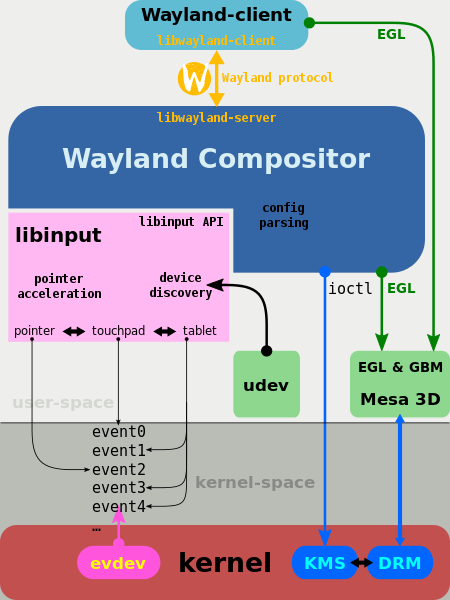
\includegraphics[width=0.7\linewidth]{waylandArchitechture}}
\caption{Архитектура протокола Wayland}
\label{fig:waylandArchitechture}
\end{figure}

Можно увидеть, что Wayland является клиент-серверным протоколом, в котором клиентами являются графические приложения, а сервером является композитор. Композитор --- это дисплейный сервер, который взаимодействует с пользовательскими устройствами ввода-вывода, с аппаратурой компьютера и управляет потоками данных клиентских приложений. В конечном счете, графические приложения запрашивают у сервера отображения своих графических буферов на экране, а композитор контролирует отображение этих буферов на экране. 

Реализация Wayland была разработана как двухслойный протокол (рис. \ref{fig:waylandClientServer}):
\begin{itemize}
\item Низкоуровневый протокол, который управляет межпроцессным взаимодействием между процессами клиента и композитора. Данный слой реализован с использованием средств ярда UNIX.
\item Поверх него построен высокоуровневый протокол, который обрабатывает информацию, которой должны обмениваться клиент и композитор для реализации базовый возможностей графической оболочки. 
\end{itemize}
\begin{figure}[h!]
\center{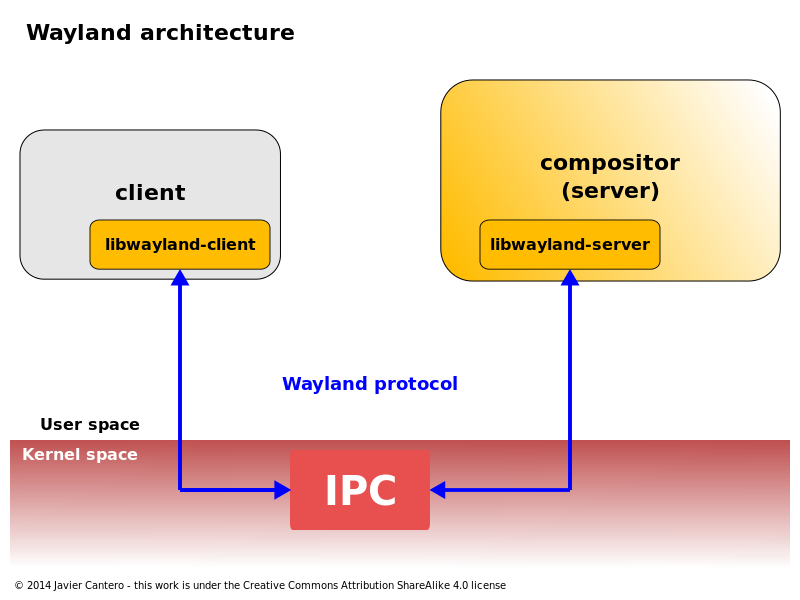
\includegraphics[width=0.7\linewidth]{waylandClientServer}}
\caption{Двухуровневая организация Wayland}
\label{fig:waylandClientServer}
\end{figure}

Реализация протокола Wayland разделена на две библиотеки: \texttt{libwayland-client} для клиентских приложений и \texttt{libwayland-server} для реализации композиторов.

Протокол Wayland описывается как "асинхронный объектно-ориентированный протокол". Объектно - ориентированность означает, что сервисы, предлагаемые композитором, представлены в виде набора объектов. Каждый объект реализует интерфейс, который имеет имя, ряд методов (называемых запросами), а также несколько связанных событий. Каждый запрос и событие имеет ноль или более аргументов, каждый из которых имеет имя и тип данных. Протокол является асинхронным в том смысле, что запросы не должны ждать синхронизированных ответов, избегая времени задержки на двустороннее сканирование. Таким образом достигается улучшенная производительность. 

Клиенты Wayland могут сделать запрос (вызов метода) для некоторого объекта, если интерфейс объекта поддерживает этот запрос. Клиент также должен предоставить необходимые данные для аргументов такого запроса. Именно так клиенты запрашивают сервисы у композитора. Композитор, в свою очередь, отправляет информацию клиенту, вызывая генерацию необходимых событий объекта. Эти события могут быть вызваны композитором как ответ на определенный запрос или асинхронно, в ответ на возникновение каких-либо внутренних событий (например, активность одного из устройства ввода). 

Для того, чтобы клиент мог сделать запрос к объекту, ему сначала нужно указать серверу идентификационный номер, который он будет использовать для идентификации этого объекта. В наборе данных есть два типа объектов: глобальные и локальные. Глобальные объекты указываются композитором клиентам, когда они созданы (а также когда они уничтожены), в то время как локальные объекты обычно создаются другими объектами, которые уже существуют как часть их функциональности. Интерфейсы, их запросы и события являются основными элементами, определяющими протокол Wayland. Каждая версия протокола включает в себя набор интерфейсов, а также их запросы и события, которые ожидаются в любом наборе Wayland. Опционально, Wayland композитор может определять и реализовывать свои собственные интерфейсы, которые поддерживают новые запросы и события, тем самым расширяя функциональность за пределами основного протокола.

Интерфейсы текущей версии протокола Wayland определены в файле протокола \texttt{protocol/wayland.xml} исходного кода Wayland. Это XML файл, в котором перечислены существующие интерфейсы текущей версии, а также их запросы, события и другие атрибуты. Этот набор интерфейсов является минимальным, необходимым для любого композитора Wayland. Некоторые из основных интерфейсов протокола Wayland:
\begin{itemize}
\item \texttt{wl\_display} --- основной глобальный объект, специальный объект для инкапсуляции самого протокола Wayland
\item \texttt{wl\_registry} --- глобальный объект реестра, в котором композитор регистрирует все глобальные объекты, которые он хочет предоставить клиентам
\item \texttt{wl\_compositor} --- объект, который представляет собой композитор, и отвечает за объединение различных буферов в один вывод
\item \texttt{wl\_surface} --- объект, представляющий прямоугольную область на экране, определяемую местоположением, размером и буфером пикселей
\item \texttt{wl\_buffer} --- объект, который при подключении к объекту \texttt{wl\_surface} предоставляет его отображаемое содержимое
\item \texttt{wl\_output} --- объект, представляющий отображаемую область экрана
\item \texttt{wl\_pointer, wl\_keyboard, wl\_touch} --- объекты, представляющие различные устройства ввода
\end{itemize} 

Типичный сеанс клиента Wayland начинается с открытия соединения с композитором с использованием объекта \texttt{wl\_display}. Это специальный локальный объект, который представляет соединение и не живет на сервере. Используя его интерфейс, клиент может запросить глобальный объект \texttt{wl\_registry} из композитора, где живут все глобальные имена объектов, и связывать те, что интересует клиента. Обычно клиент связывает по крайней мере объект \texttt{wl\_compositor}, откуда он будет запрашивать один или несколько объектов \texttt{wl\_surface} для отображения вывода приложения на дисплее.

Композитор Wayland может определять и экспортировать свои собственные дополнительные интерфейсы. Эта функция используется для расширения протокола за пределами базовых функций, предоставляемых основными интерфейсами, и стала стандартным способом реализации расширений протокола Wayland.

Для Wyaland так же существует расширение XWayland, которое позволяет запускать X-приложения в Wayland.

\subsection{Сравнение X и Wayland}
Существует несколько отличий между Wayland и X в отношении производительности, поддержки кода и безопасности: 
\begin{itemize}
\item Архитектура: композитор --- это отдельная дополнительная функция в X, а Wayland объединяет дисплейный сервер и композитор как единую функцию. Кроме того, он включает в себя некоторые из задач оконного менеджера, который в X является отдельным процессом на стороне клиента. 
\item Рендеринг: X-сервер по-умолчанию сам выполняет рендеринг окон. Существуют так же расширения позволяющие ему окно отрендеренное на стороне клиента. Напротив, Wayland по-умолчанию не предоставляет API для визуализации, а делегирует клиентам такие задачи (включая рендеринг шрифтов, виджетов и т. д.). Декорирование окон может выполняться на клиентской стороне (например, с помощью набора графических средств) или на стороне сервера (в функциональности композитора). 
\item Безопасность: Wayland изолирует входные и выходные данные каждого окна, обеспечивая конфиденциальность, целостность и доступность в обоих случаях; X не имеет этих важных функций безопасности. Кроме того, с подавляющим большинством кода, работающего на клиенте, меньше кода нужно запускать с правами root, что повышает безопасность. 
\item Межпроцессное взаимодействие: X-сервер предоставляет базовый метод обмена между X-клиентами, позднее расширенный протоколом ICCM. Это взаимодействие X клиент --- X клиент используется менеджерами окон, для реализации X-сессий, функций drag-and-drop, а многих других функций. Основной протокол Wayland не поддерживает связь между wayland-клиентами вообще, и соответствующая функциональность (если необходимо) должна быть реализована в окружении рабочего стола (например, KDE или GNOME) или третьей стороной (например, используя IPC базовая операционной системы).
\item Сетевое взаимодействие: X --- это архитектура, изначально разработанная для работы по сети. Wayland не предлагает сетевой прозрачности сам по себе, однако, композитор может реализовать любой протокол удаленного рабочего стола для достижения удаленного отображения. Кроме того, существуют исследования потоковой передачи и сжатия изображений Wayland, которые обеспечивали бы доступ к буферу буфера удаленного доступа, подобный VNC.
\end{itemize}

На основе всех этих фактов можно сказать, что Wayland является более современной графической средой, в которой учтены и исправлены многие ошибки X. Благодаря этому, Wayland так же выигрывает у X в производительности. Wayland так же поддерживает X-приложения (через XWayland). Таким образом, можно сделать вывод, что наиболее оптимальным выбором для реализации своего мобильного оконного менеджера будет выбор Wayland.

	\section{Анализ существующих композиторов Wayland}
\subsection{Weston}
Weston --- это референсная реализация композитора Wayland. Weston поставляется с несколькими примерами клиентов, от простых, которые демонстрируют некоторые аспекты протокола для, до полных клиентов и упрощенного инструментария. Существует также полноценный эмулятор терминала (weston-terminal) и простая оболочка рабочего стола. Наконец, Weston также обеспечивает интеграцию с сервером Xorg и может разместить X-клиенты на рабочем столе Wayland и представляться им как ОМ X. Пример запуска Weston привежен на рисунке \ref{fig:weston}.

\begin{figure}[h!]
\center{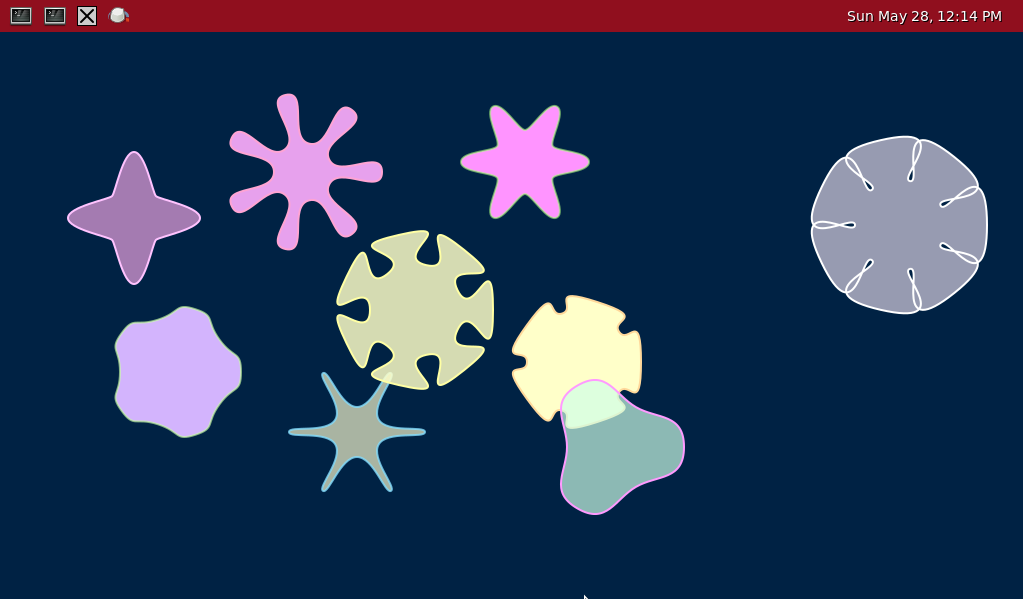
\includegraphics[width=\linewidth]{weston}}
\caption{Рабочий стол Weston}
\label{fig:weston}
\end{figure}

Weston по умолчанию поддерживает несколько бекендов, что позволяет ему без проблем запускаться на большом количестве платформ. До версии 1.9 Weston так же поддерживал бекенд для проприетарной графической системы Raspberry Pi, однако разработчики отказались от этой части из-за сложности поддержки кода.

Пакет Weston по умолчанию включает в себя библиотеку libweston. Libweston --- это попытка отделить переиспользуемый исхдный код Weston в отдельную библиотеку. Эта библиотека включает в себя корректную реализацию всех базовых протоколов Wayland и взаимодействие с подсистемами ввода вывода. Libweston предлагается использовать для облегчения разработки собственных ОМ.

Libweston впервые появился в версии Weston 1.12. В настоящее время библиотека находится в состоянии активной разработки. Разработчики утверждают, что API библиотеки не стабилен может сильно изменяться от версии к версии, поэтому в данный момент использование этой библиотеки не самое лучшее решение. 

\subsection{WLC}
WLC --- популярная библиотека-композитор для Wayland~\cite{wlc}. На основе этой библиотеки реализовано несколько оконных менеджеров и других библиотек. Их примеры:
\begin{itemize}
\item Тайлинговый оконный менеджер Sway (рис.~\ref{fig:sway})
\item Модульный композитор orbment
\item Модульный ОМ fireplace
\end{itemize}

\begin{figure}[h!]
\center{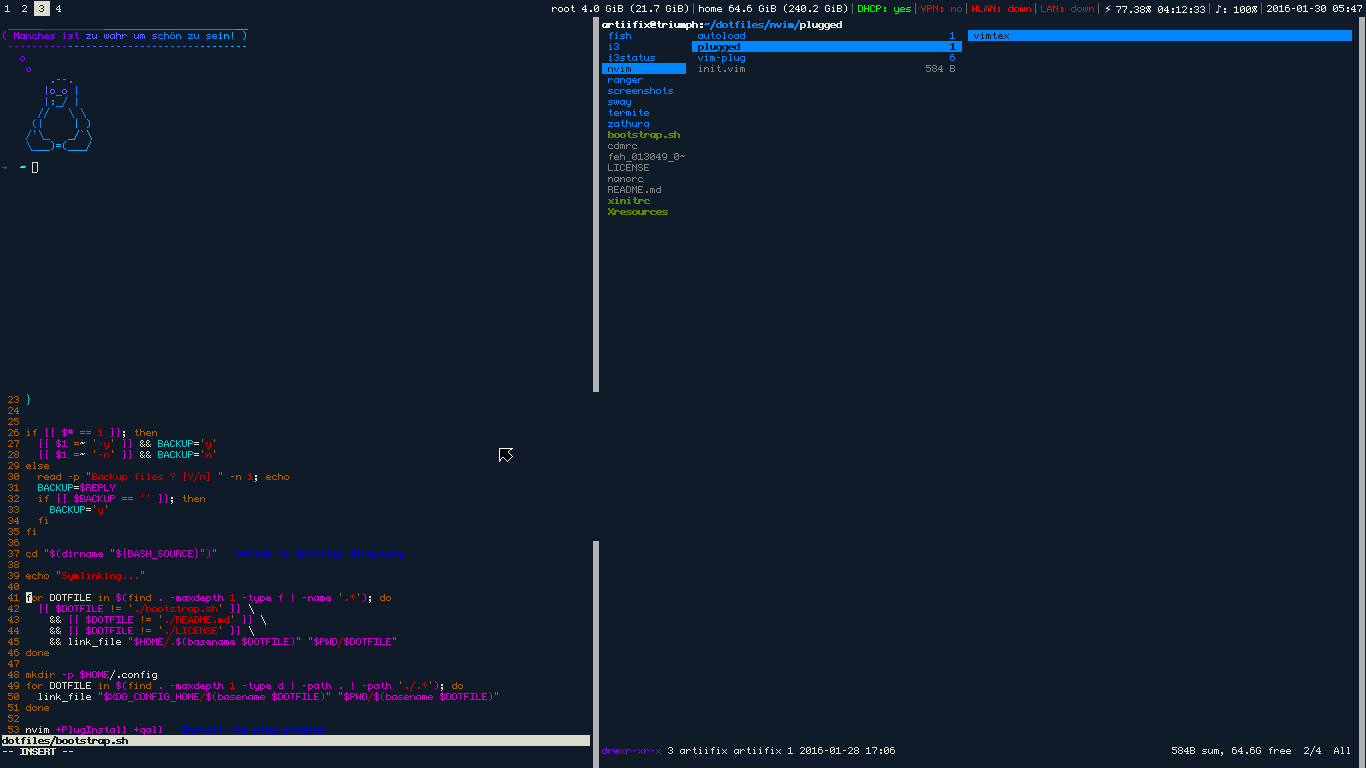
\includegraphics[width=\linewidth]{sway}}
\caption{Пример Sway}
\label{fig:sway}
\end{figure}

Библиотека обладает большой функциональностью. Она поддерживает различные бекенды, может запускаться как под X11, так и под Wayland. Библиотека очень удобна для разработки на ее основе собственного ОМ, так как она содержит примеры написания простейших ОМ.

\subsection{SWC}
SWC --- это небольшой композитор Wayland, реализованный в виде библиотеки. Разработчик SWC утверждает, что swc был написан с целью предоставить минимальный набор функций для возможности отображения окон на экране.

На основе SWC реализован простой оконный менеджер Velox, предназначение которого --- продемонстрировать возможности библиотеки.

\begin{figure}[h!]
\center{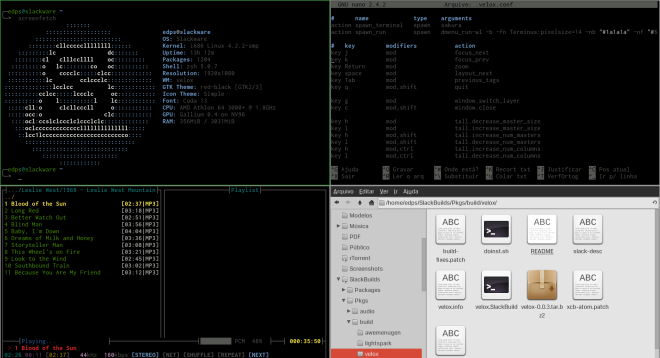
\includegraphics[width=\linewidth]{velox}}
\caption{ОМ Velox}
\label{fig:velox}
\end{figure}


	\section{Выполнение работы}
\subsection{Описание тестового стенда}
Для выполнения работы использовалось два тестовых стенда:
\begin{itemize}
\item Платформа Raspberry Pi 1 с ОС ArchLinux
\item Виртуальная машина с Arch Linux
\end{itemize}

Благодаря тому, что платформы Raspberry Pi 1 и Raspberry Pi Zero аппаратно полностью совместимы, ОМ разработанный на платформе RPi 1 будет совместим с RPi Zero. Однако, проблема в том, что RPi имеет проприетарную графику, которая не поддерживается в Wayland. Поэтому, задача конфигурирования ОС на платформе RPi включала в себя установку драйвера VC4~\cite{vc4}, который позволяет представить видеокарту RPi как стандартное DRI устройство.

Виртуальная машина c ArchLinux была установлена в гипервизоре VirtualBox. Однако, из-за того что в VirtualBox не реализована поддержка протокла Wayland, мобильный оконный менеджер запускался в качестве X-клиента в оконном менеджере xfce4.

\subsection{Выбор библиотеки-композитора}
Как было сказано ранее, в архитектуре Wayland оконный менеджер обязательно должен включать в себя композитор (в отличие от X). Так как реализация собственного Wayland-композитора с нуля --- задача слишком объемная и трудоемкая, был решено использовать какую-либо библиотеку-композитор. В таком случае задачей разработанного ОМ будет управление окнами.

Из проанализированных библиотек было решено выбрать библиотеку wlc по нескольким причинам:
\begin{itemize}
\item API библиотеки устойчив и проверен
\item на ее основе уже реализовано некоторое количество программ
\item для библиотеки есть некоторое количество примеров
\end{itemize}

\subsection{Разработка оконного менеджера}
Исходный код основного файла оконного менеджера приведен в листинге~\ref{lst:main}. В основной функции приложения main производятся следующие действия:
\begin{itemize}
\item анализируются аргументы командной строки (строки 358-365)
\item считывается конфигурация (строка 367)
\item устанавливаются функции-обработчики действий для wlc (строки 370-392)
\item инициализируется композитор (строки 395-397)
\item запускаются системные приложения (строка состояния и рабочий стол) (строки 399-425)
\item запускается оконный менеджер (строка 426)
\end{itemize}

Созданное приложение принимает один аргумент --- файл конфигурации. Если аргумент не указан, ищется и открывается файл по-умолчанию -- \texttt{~/.config/xxwm}. Пример конфигурационного файла приведен в листинге \ref{lst:conf}. В нем указываются пути к исполняемым файлам строки состояния и рабочего стола.

\begin{lstlisting}[label=lst:conf, caption={Формат конфигурационного файла ОМ}]
[statusbar]
exe=/home/kivi/workspace/Phone/src/status_bar/status

[desktop]
exe=/home/kivi/workspace/Phone/src/desktop/desktop
\end{lstlisting}

Считывание конфигурационного файла производится с помощью библиотеки inih. Исходные коды функций, которые производят считывание конфигурационного файла приведены в листингах \ref{lst:confh} -- \ref{lst:confc}.

Далее в функции main устанавливаются функции-обработчики для библиотеки-композитора. Данные функции обрабатывают события, получаемые от композитора и, соответственно, работают с типами данных композитора.  Композитор определяет несколько абстракций:
\begin{itemize}
\item output --- вся область отображения на экран. В терминах оконных менеджеров это соответствует "рабочему столу"
\item view --- окно приложения
\end{itemize}

Рассмотрим все эти функции более подробно.
\begin{itemize}
\item \texttt{wlc\_log\_set\_handler} устанавливает функцию, которая будет осуществлять логирование. В нашем случае устанавливается функция, которая просто выводит все сообщения в терминал с использованием функции \texttt{printf} (строчки 352-355).

\item \texttt{wlc\_set\_output\_resolution\_cb} устанавливает функцию, которая обрабатывает изменение разрешения экрана. Устанавливаемая функция \texttt{output\_resolution} просто вызывает функцию перерисовки окон \texttt{relayout} (строчки 174-177).

\item \texttt{wlc\_set\_view\_created\_cb} устанавливает функцию, которая будет вызываться при создании нового окна. Устанавливаемая функция \texttt{view\_created} устанавливает окну необходимые флаги, выносит окно на первый план, переключает фокус на это окно и вызывает функцию перерисовки (строки 180-192).

\item \texttt{wlc\_set\_view\_destroyed\_cb} устанавливает функцию, которая будет вызваться при уничтожении окна. Устанавливаемая функция \texttt{view\_destroyed} устанавливает фокус на самое верхнее окно и вызывает функцию перерисовки (строки 195-200).

\item \texttt{wlc\_set\_view\_focus\_cb} устанавливает функцию, которая отвечает за установку фокуса на окно. Устанавливаемая функция \texttt{view\_focus} устанавливает окну флаг \texttt{WLC\_BIT\_ACTIATED} (строчки 203-206).

\item \texttt{wlc\_set\_view\_request\_move\_cb} устанавливает функцию, которая отвечает за перемещение какого-либо окна по экрану. Устанавливаемая функция \texttt{view\_request\_move} вызывает функцию \texttt{start\_interactive\_move} (строчка 210), которая в свою очередь начинает интерактивное действие вызвав функцию \texttt{start\_interactive\_action} (строчка 42).  Функция \texttt{start\_interactive\_action} сохраняет параметры окна, на котором начато интерактивное действие, в глобальную переменную и выводит это окно на первый план (строчки 26-38).

\item \texttt{wlc\_set\_view\_request\_resize\_cb} устанавливает функцию, которая отвечает за изменение размеров окна. Устанавливаемая функция \texttt{view\_request\_resize} начинает интерактивное действие изменения окна вызывая функцию \texttt{start\_interactive\_resize} (строчка 215). Данная функция начинает интерактивное действие вызвав функцию \texttt{start\_interactive\_action}, а затем определяет то, какую грань окна необходимо перемещать (строчки 46-66). Так же данная функция устанавливает окну флаг \texttt{WLC\_BIT\_RESIZING}, который указывает на то, что окно в текущий момент меняет свой размер.

\item \texttt{wlc\_set\_view\_request\_geometry\_cb} устанавливает функцию, которая отвечает за установку указанному окну определенных размеров. Устанавливаемая функция \texttt{view\_request\_geometry} не делает ничего, так как ОМ не предполагает возможности изменять размер окна извне.

\item \texttt{wlc\_set\_keyboard\_key\_cb} устанавливает функцию-обработчик нажатий клавиатуры. Устанавливаемая функция \texttt{keyboard\_key} считывает код нажатой клавиши, флаги модификаторов (CTRL, ALT и т.д.) и обрабатывает следующие комбинации (строчки 225-266):
\begin{itemize}
\item CTRL+q --- закрытие активного окна (если это не системное приложение)
\item CTRL+стрелка вниз --- переключиться на следующее окно (аналог ALT+Tab в Windows)
\item CTRL+Escape --- завершить работу оконного менеджера
\item CTRL+Enter --- запустить терминал
\end{itemize}

\item \texttt{wlc\_set\_pointer\_button\_cb} устанавливает функцию-обработчик нажатий кнопок мыши. Устанавливаемая функция \texttt{pointer\_button} обрабатывает следующие комбинации (строчки 268-291):
\begin{itemize}
\item CTRL+ЛКМ --- переместить окно
\item CTRL+ПКМ --- изменить размеры окна
\end{itemize}

\item \texttt{wlc\_set\_pointer\_motion\_cb} устанавливает функцию-обработчик передвижения мыши. Устанавливаемая функция \texttt{pointer\_motion} проверяет, если в данный момент выполняется интерактивное действие, она соответствующим образом изменяет отображение активного окна (передвигает или изменяет размеры, в зависимости от выполняемого действия) (строчки 294-350).
\end{itemize}

Далее в функции main выполняется запуск системных приложений (строки состояния и рабочего стола) и запуск самого композитора. При этом, ОМ запоминает PID системных приложений для возможности их идентификации. Например, на основе этих PID ОМ решает можно ли закрывать соответствующее окно.

Одной из самых главных функций ОМ является функция перерисовки окно \texttt{relayout} (строки 90-171). Данная функция действует по следующему алгоритму:
\begin{enumerate}
\item берет самое верхнее (переднее) окно
\item проверяем, является ли окно окном строки состояния
\item если да, то запоминаем идентификатор окна
\item если нет, то рисуем данное окно на весь экран, кроме верхней строчки высотой в 30 пикселей
\item обновляем окно строки состояния перерисовывая ее в верхних 30 пикселях экрана 
\end{enumerate}

Данный алгоритм позволяет каждый раз перерисовывать максимум два окно: активное окно приложения и окно строки состояния. Строку состояние необходимо перерисовывать, потому что в какой-то момент времени могло изменится разрешение экрана. Данный алгоритм позволяет снизить вычислительную нагрузку ОМ на систему. 

Так же при перерисовке окна учитываются флаги типа окна. Библиотека WLC определяет пять флагов окна. Экспериментальным путем было выяснено, что при работе ОМ появляются и должны по-особому отображаться только два типа окон:
\begin{itemize}
\item \texttt{WLC\_BIT\_UNMANAGED} --- окна меню
\item \texttt{WLC\_BIT\_POPUP} --- уведомления и контекстные меню (вызываемые при нажатии ПКМ)
\end{itemize}

Данные типы окон отображаются по-особому. Окна меню отображаются в соответствии с изначально заданными им параметрами, ничего не изменяется. Окна контекстных меню смещаются относительно координат их окна-родителя и координат нажатия мыши. Остальные окна отображаются по-умолчанию на всю область экрана, незанятую строкой состояния.

Примеры работы оконного менеджера приведены на рисунках \ref{fig:wm1} -- \ref{fig:wm4}.
\begin{figure}[h!]
\center{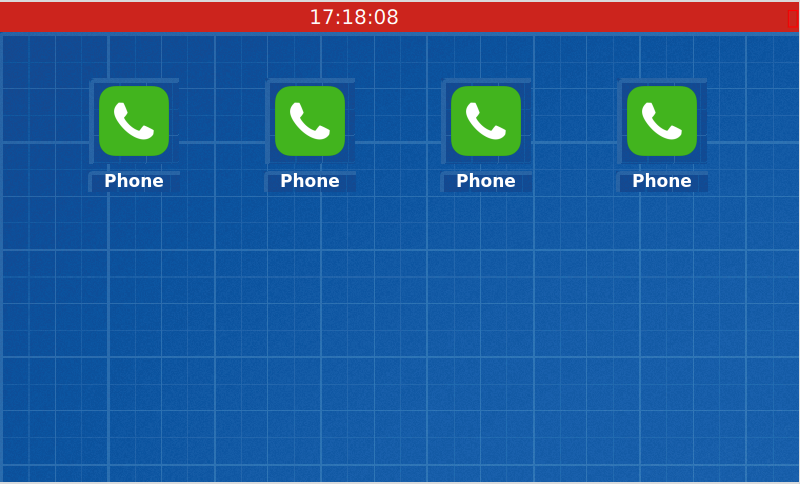
\includegraphics[width=\linewidth]{wm1}}
\caption{Оконный менеджер}
\label{fig:wm1}
\end{figure}
\begin{figure}[h!]
\center{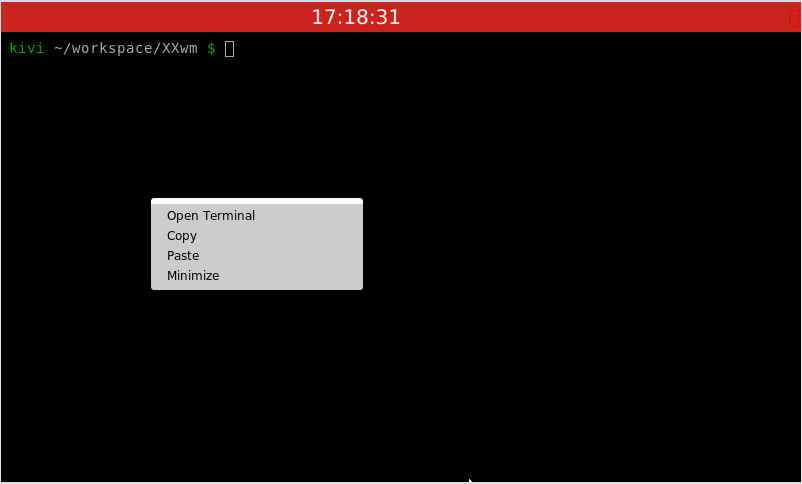
\includegraphics[width=\linewidth]{wm2}}
\caption{Отображение терминала и контекстного меню}
\label{fig:wm2}
\end{figure}
\begin{figure}[h!]
\center{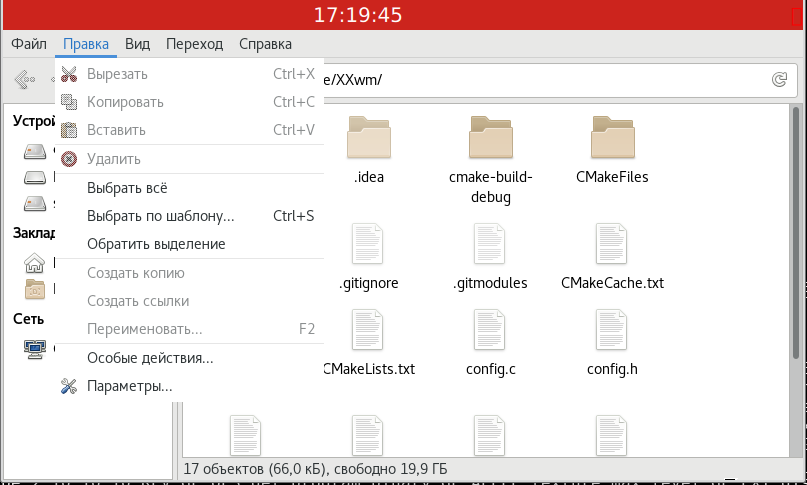
\includegraphics[width=\linewidth]{wm3}}
\caption{Отображение файлового менеджера и меню}
\label{fig:wm3}
\end{figure}
\begin{figure}[h!]
\center{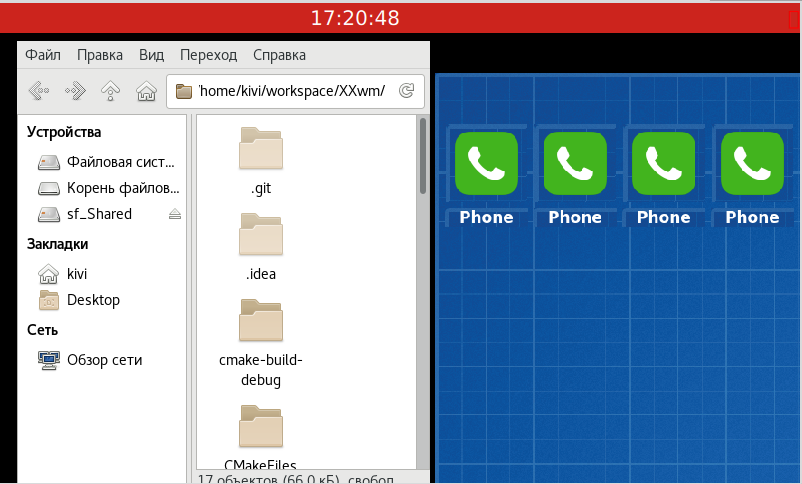
\includegraphics[width=\linewidth]{wm4}}
\caption{Перемещение и изменение размеров окон}
\label{fig:wm4}
\end{figure}

\subsection{Добавление ОМ в экранный менеджер}
Экранный менеджер или менеджер входа --- графический экран, который отображается в конце процесса загрузки вместо стандартного приглашения командной строки. Экранный менеджер представляет собой экран ввода имени пользователя и пароля для входа в систему. Существует большое количество экранных менеджеров, однако все они детектируют установленные в систему оконные менеджеры по конфигурационным файлам формата \texttt{.desktop}. Данные файлы являются неким подобием ярлыков в Windows. \texttt{.desktop} --- это сандартный для Linux конфигурационный файл. Подробное описание формата файлов \texttt{.desktop} приведено в~\cite{desktop}. Для созданного ОМ был создан минимальный файл \texttt{.desktop} (листинг \ref{lst:desktop}).
\begin{lstlisting}[label=lst:desktop, caption={Файл .desktop для ОМ}]
[Desktop Entry]
Name=XXwm
Comment=Mobile Wayland window manager
Exec=/home/kivi/workspace/XXwm/xxonwm
Type=Application
\end{lstlisting}

Для того, чтобы экранный менеджер смог обнаружить ОМ необходимо поместить \texttt{.desktop} в каталог \texttt{/usr/share/wayland-sessions/}. Для проверки данного файла был установлен экранный менеджер sddm. Пример выбора ОС в sddm приведен на рисунке \ref{fig:sddm}.
\begin{figure}[h!]
\center{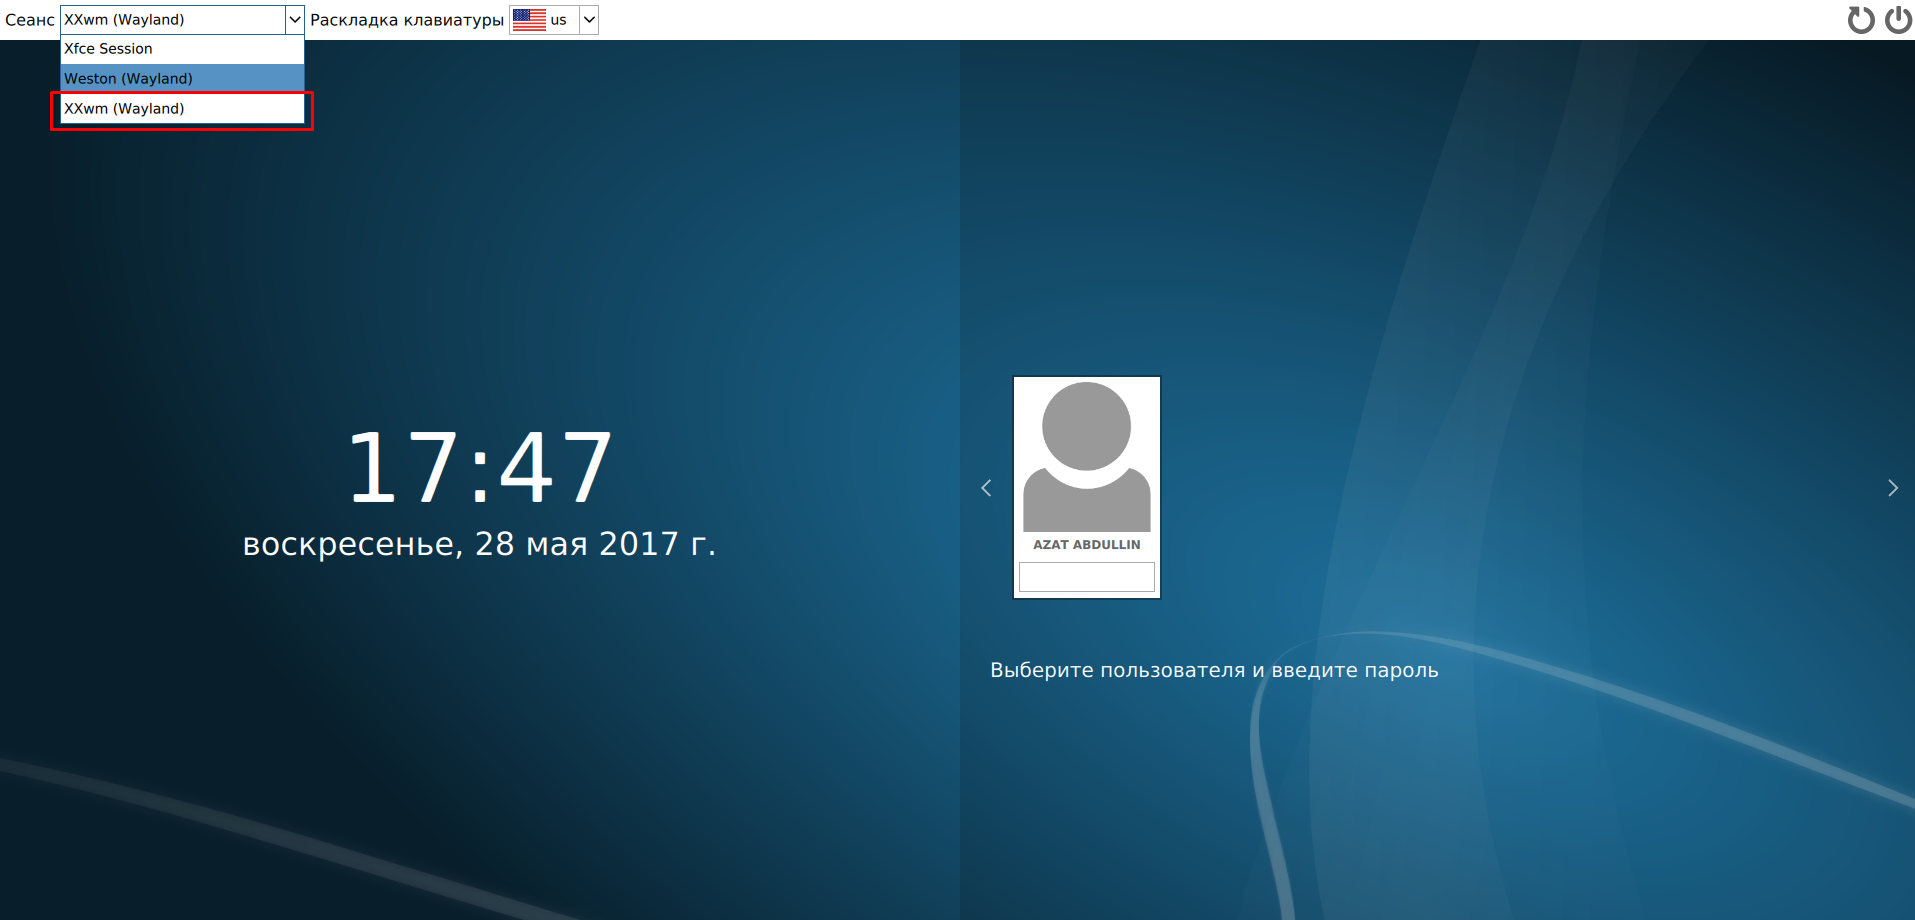
\includegraphics[width=\linewidth]{sddm}}
\caption{Пример загрузки ОМ через экранный менеджер}
\label{fig:sddm}
\end{figure}
	\section{Выводы}
В ходе работы были проанализированы и сравнены протоколы организации графических серверов в UNIX-подобных системах. В результате анализа было решено, что Wayland является более современной и оптимальной системой для разработки мобильного оконного менеджера.
В данной работе был реализован мобильный оконный менеджер для протокола Wayland. Данный оконный менеджер разрабатывался в рамках проекта по разработке мобильного телефона. Разработанный оконный менеджер позволяет запускать системные приложения (строка состояния и рабочий стол) и обычные пользовательские приложения. Оконный менеджер так же обрабатывает несколько комбинаций клавиш для управления окнами, а так же позволяет перемещать окна и изменять из размеры с помощью   мыши.
	\FloatBarrier
			
	\pagebreak
	\addcontentsline{toc}{section}{Список используемой литературы}
	\bibliography{biblio}
	\bibliographystyle{ugost2008}  %% стилевой файл для оформления по ГОСТу
	
	\pagebreak	
	\section{Прилагаемые материалы}
	Все прилагаемые материалы находятся в папке man.
	Список прилагаемых материалов следующий:
	\begin{itemize}
		\item Техническое задание.docx --- техническое задание на проект;
		\item programmingGuilde.pdf --- руководство системного программиста;
		\item programText.pdf --- текст программы;
		\item spec.pdf --- описание программы;
		\item testGuide.pdf --- программа и методика испытаний;
		\item userGuide.pdf --- руководство пользователя.
	\end{itemize}
	Так же прилагается пояснительная записка (report/report.pdf).
	
	
	\pagebreak
	\section*{Листинги}

\lstinputlisting[label=lst:main, caption={Файл main.c}, 
language={C}]{../src/main.c}

\lstinputlisting[label=lst:confh, caption={Файл config.h}, 
language={C}]{../src/config.h}

\lstinputlisting[label=lst:confc, caption={Файл config.c}, 
language={C}]{../src/config.c}

\lstinputlisting[label=lst:cmake, caption={Файл сборки CMakeLists.txt}, 
language={C}]{../src/CMakeLists.txt}
\end{document}